Memory-efficient Zeroth-order Optimizer (MeZO):

\begin{itemize}
    \item At each training step, does two forward passes with different amounts of perturbation on parameters
    \item Estimates gradients using only those forward passes (no backpropagation)
    \item Very memory-efficient but high computation time
    %\item Can be used in combination with other PEFT methods
    %\item Requires prompt-based fine-tuning
    \item Works under a prompt-based fine-tuning setting
\end{itemize}

\begin{figure}
    \centering
    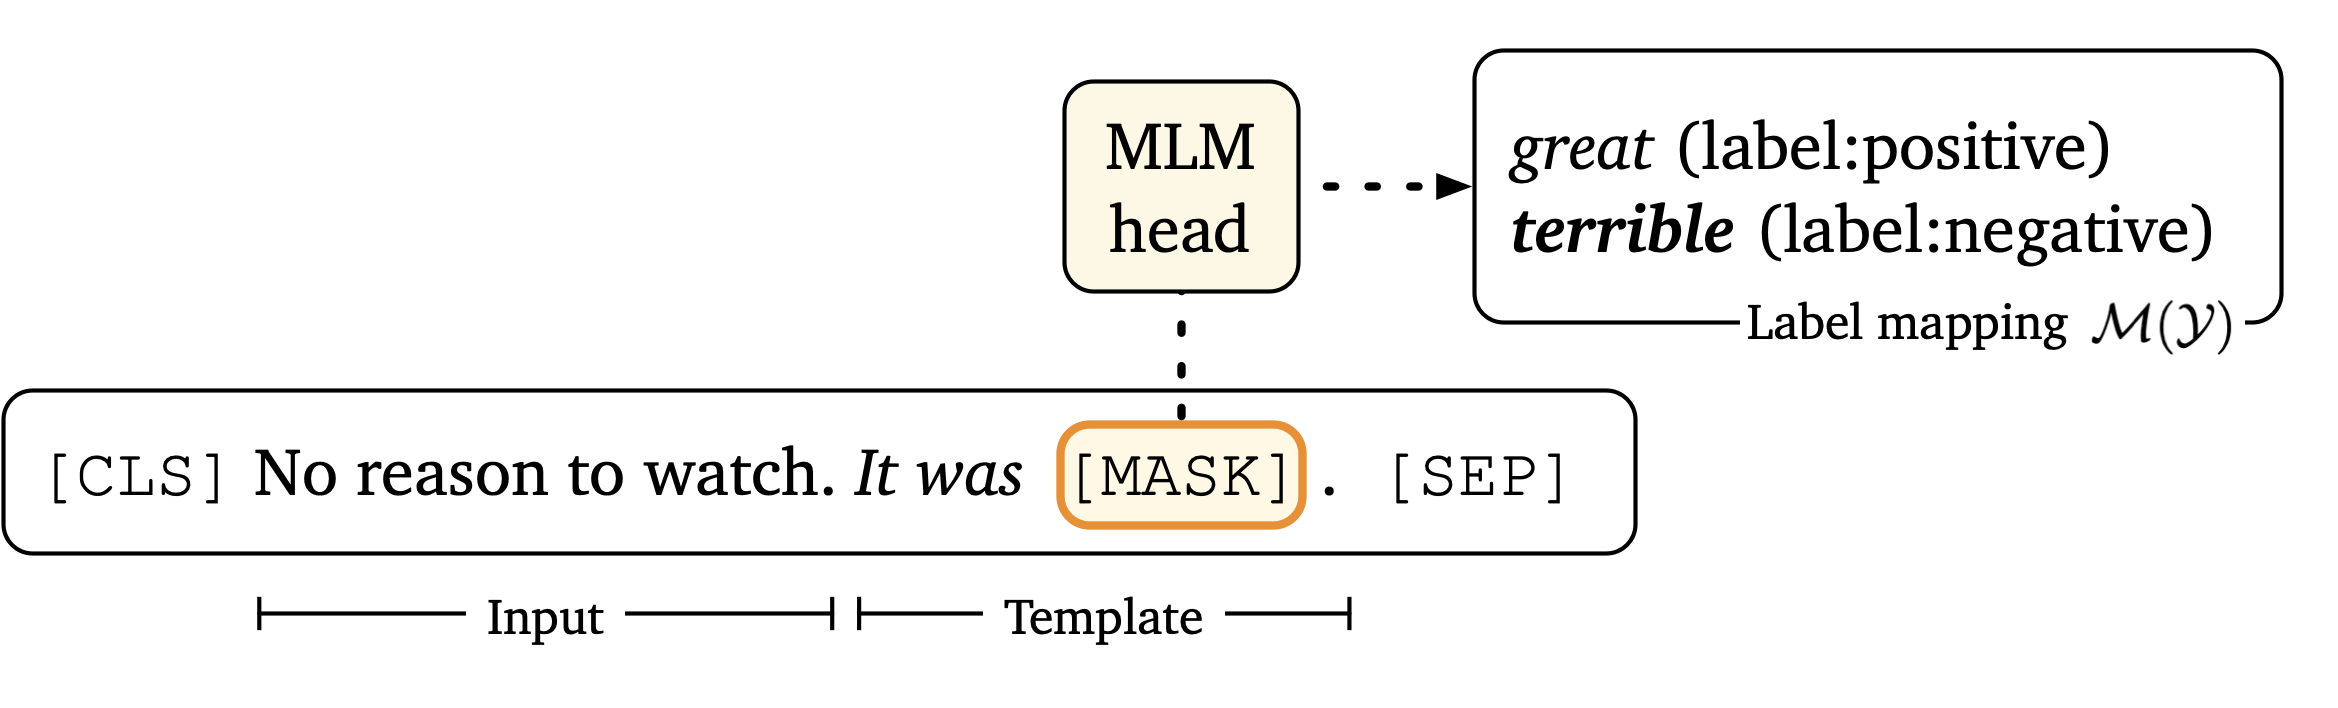
\includegraphics[width=\textwidth]{assets/images/Prompt.png}
    \caption{Prompt-based Fine-tuning}
    \label{fig:prompt}
\end{figure}

\textbf{Some MeZO Ideas:}
\begin{itemize}
    \item Before training with LST, fine-tune backbone model using MeZO
    \item Fine-tune entire model using MeZO, then fine-tune last few layers with backpropagation. 
\end{itemize}

\textbf{Experiment Results:}
\begin{itemize}
    \item Adding a prompt to input sentences improves performance for both LST and layer freezing
    %\item Training with MeZO beforehand seems to be irrelevant for the improvement.
    \item Only the added prompt seems to be relevant for this improvement and not the prior training with MeZO.
    \item The choice of prompt has a significant impact on the performance gains.
\end{itemize}
